\documentclass[11pt]{article}

\usepackage{fullpage}
\usepackage{graphicx}
\usepackage{amsmath}
\usepackage{amssymb}
\usepackage{amsthm}
\usepackage{fancyvrb}

\parindent0in
\pagestyle{plain}
\thispagestyle{plain}

\newcommand{\myname}{Mehshan Mustafa}
\newcommand{\dated}{\today}

\newenvironment{theorem}[2][Theorem]{\begin{trivlist}
\item[\hskip \labelsep {\bfseries #1}\hskip \labelsep {\bfseries #2.}]}{\end{trivlist}}
\newenvironment{lemma}[2][Lemma]{\begin{trivlist}
\item[\hskip \labelsep {\bfseries #1}\hskip \labelsep {\bfseries #2.}]}{\end{trivlist}}
\newenvironment{exercise}[2][Exercise]{\begin{trivlist}
\item[\hskip \labelsep {\bfseries #1}\hskip \labelsep {\bfseries #2.}]}{\end{trivlist}}
\newenvironment{problem}[2][Problem]{\begin{trivlist}
\item[\hskip \labelsep {\bfseries #1}\hskip \labelsep {\bfseries #2.}]}{\end{trivlist}}
\newenvironment{question}[2][Question]{\begin{trivlist}
\item[\hskip \labelsep {\bfseries #1}\hskip \labelsep {\bfseries #2.}]}{\end{trivlist}}
\newenvironment{corollary}[2][Corollary]{\begin{trivlist}
\item[\hskip \labelsep {\bfseries #1}\hskip \labelsep {\bfseries #2.}]}{\end{trivlist}}
\newenvironment{solution}{\begin{proof}[Solution]}{\end{proof}}
\newenvironment{idea}[2][Proof Idea.]{\textit{#1} #2}

\begin{document}

\textbf{Introduction to the Theory of
Computation}\hfill\textbf{\myname}\\[0.01in]
\textbf{Chapter 1: Reqular Languages}\hfill\textbf{\dated}\\
\smallskip\hrule\bigskip

\begin{problem}{1.46}
Prove that the following languages are not regular. You may use the pumping
lemma and the closure of the class of regular languages under union, intersection, and complement.
\end{problem}

\begin{problem}[Part]{c}
$\{w \ | \ w \in \{0,1\}^{*} \ is \ not \ a \ palindrome\}$
\end{problem}

\begin{proof}
The proof is by contadiction. Assume $A$ is a regular language. Let $p$ be the pumping lenght given by the pumping lemma. Let $s$ be the string:
\[ s = 0^{p}10^{p+p!} \]
The string $s$ is a member of $A$, and $|s| \geq p$, therefore the pumping lemma guarantees that $s$ can be split into three pieces, $s = xyz$, where for any $i \geq 0$ the string $xy^{i}z \in A$. According to the condition 3 $(|xy| \leq p)$ of the pumping lemma, $y$ consists of 0s. Let $m+n = p$, where $0 \leq m < p$ and $1 \leq n \leq p$. Then
\[ 0^{m} \Bigl[0^{n}\Bigr]^{i}10^{p+p!} \in A. \]
But for $i = 1 + \frac{p!}{n}$, the number of 0s on both sides of the 1 become the same and the resulting string is a palindrome, which is a contradiction.
\end{proof}

\begin{problem}[Part]{d}
$\{wtw \ | \ w, \ t \in \{0,1\}^{+}\}$
\end{problem}

\begin{proof}
The proof is by contradiction. Assume $A$ is a regular language. Let $p$ be the pumping length give by the pumping lemma. Choose $w = 1^{p}0$ and $t=0$, so the string $s$ is:
\[ s = 1^{p}001^{p}0 \]
The string $s$ is a member of $A$, $|s| \geq p$, therefore the pumping lemma guarantees that the string $s$ can be split into three pieces, $s=xyz$, where for any $i \geq 0$ the string $xy^{i}z \in A$. According to the condition 3 of the pumping lemma, $y$ can only contain 1s. More specfically, $y$ can contain any number of 1s from 1 to $p$. Also, it must be the case that $w$ starts with 1 and ends with a 0. When $i > p$, there are more 1s at the start of $s$ then the number of 1s before the last 0, so there is no way to pick a $w$. Therefore, $xy^{p+1}z \notin A$, which is a contradiction.
\begin{center}
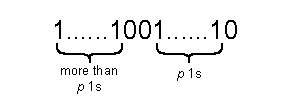
\includegraphics[scale=2.0]{Figures/Problem1.46.pdf} \\
When $i > p$, there are more 1s at the start of $s$.
\end{center}
\end{proof}

\end{document}